\graphicspath{{graphical-models/}}

\chapter{Graphical Models}

There are numerous formalisms for representing informational relationships
between variables using shapes connected by lines or arrows (illustrated in
fig.~\ref{fig:bayes}). In this proposal, when I describe something as a
graphical model, I mean specifically that it is a directed Bayesian graphical
model (sometimes referred to as a ``Pearl net'' or a ``Bayes net''). Here I will use
``Bayes net'' for brevity.  There are two reasonable points of departure in
describing this formalism.

\begin{figure}
\begin{center}
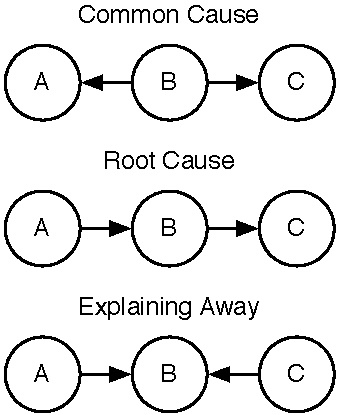
\includegraphics{bayes-nets.pdf}
\end{center}
\caption{A set of simple Bayes nets that illustrate the 3 topologies for a
    3-node, 2-link network.}
\label{fig:bayes}
\end{figure}

\section{Starting with SEM}

If you are familiar with the Structural Equation Modelling (SEM) formalism,
Bayes nets are quite similar, but differ in two
important ways. If you are \emph{not} familiar with SEM, please skip to the
following section. First, while SEM is a normal theory model (which allows for
relatively efficient estimation of parameters), each variable in a Bayes net may
have an arbitrary distribution. Sometimes pragmatic constraints are
placed upon these distributions, for example that they must come from the
exponential family. For their more descriptive useage in the proposal, such
constraints are unnecessary. A second difference is that the bidirectional arrows
signifying correlations in SEM are unavailable.

\section{Conditional independence}

Bayes nets are an easily human-interpretable representation of the conditional
dependencies (or lack thereof) between variables. In particular, there may be
(and usually is) a dependence between any two variables (nodes) in a Bayes net
if you are able to trace a path first up some set of arrows, and then down
another set. Thus, in fig.~\ref{fig:bayes}, A is independent of C only in the
``explaining away'' variation, where you can only reach C from A by going first
down, then up an arrow. Formally, a variable A is independent of B iff 
$p(A|B) = p(A)$.

Moreover, if the only way to get from A to C is via an intervening node B (or set
of intervening nodes), then A is conditionally independent of C given B. This is
the case in all three examples in fig.~\ref{fig:bayes}. Formally, 
$p(A|B,C) = p(A|B)$.
